

\fancypagestyle{miEstilo7}{
   \lhead{7. Conclusión y trabajos futuros}
   \rhead{Página \thepage}
   \lfoot{}
   \cfoot{}
   \rfoot{}
}

\pagestyle{miEstilo7}

\section{Conclusiones y trabajos futuros}\label{sec:conclusiones}

Tras finalizar, puedo concluir que este proyecto ha sido un éxito personal y se han cumplido satisfactoriamente los objetivos propuestos al inicio del proyecto. El resultado obtenido ha sido un sistema de videovigilancia de bajo coste, que es capaz de alertas a los usuarios ante eventos de movimiento, y con capacidad de monitorizar el estado de un entorno para aumentar su nivel de seguridad.

En cuanto a la planificación, decir que se ha cumplido con la planificación prevista. Se han implementado el conjunto de funcionalidades indicadas en el plazo establecido. La planificación que se previó fue un poco pesimista, es decir, el proyecto se ha conseguido desarrollar en menos tiempo del esperado. En concreto, \textbf{el número de horas que se estimó al inicio del proyecto fue de 341h y finalmente se ha desarrollado en 267h}. Hay que destacar que esta diferencia se debe a la incertidumbre inicial, ya que muchas herramientas y tecnologías eran desconocidas y se estimó un tiempo al alza por si el periodo de adaptación era más costoso.

De hecho, en las siguientes figuras podemos comparar el diagrama de Gantt que se propuso al iniciar el proyecto y el diagrama de Gantt obtenido tras finalizar el proyecto.

\begin{figure}[h]
	\centering
	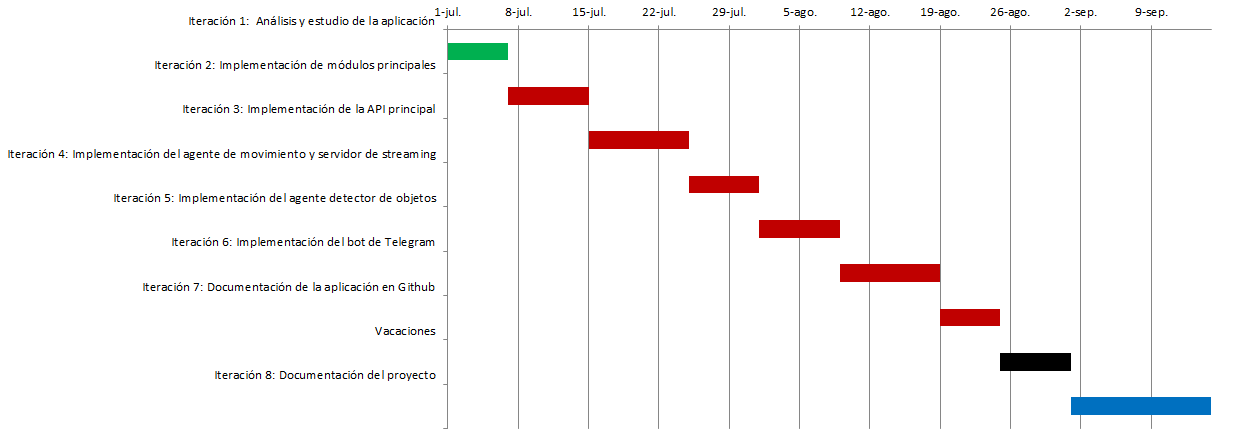
\includegraphics[scale=0.45]{images/diagrama_gantt}
	\caption{Diagrama de Gantt del proyecto previsto}
\end{figure}

\newpage

\begin{figure}[h]
	\centering
	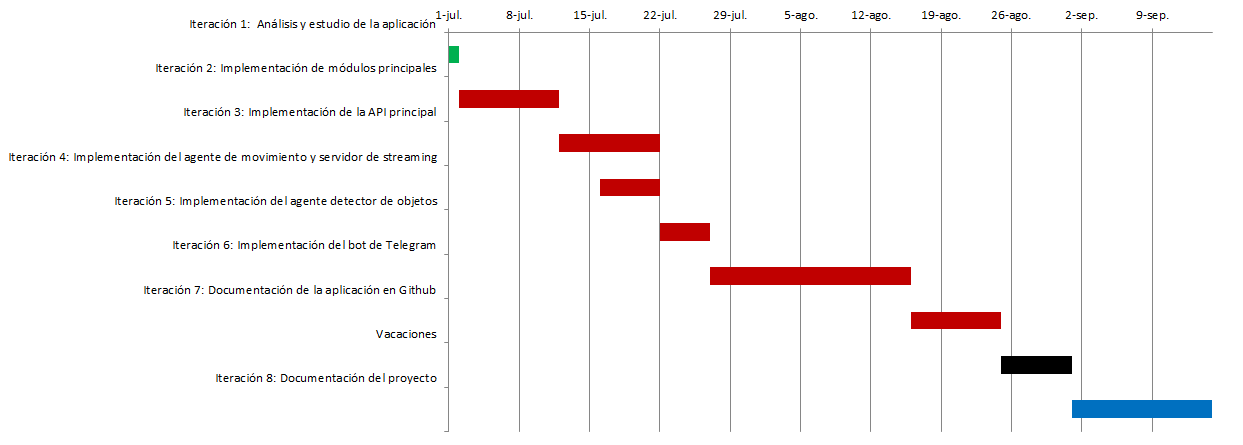
\includegraphics[scale=0.45]{images/diagrama_gantt_real}
	\caption{Diagrama de Gantt del proyecto real}
\end{figure}

Como se puede observar, ha habido algunas diferencias entre ambos. En primer lugar, la primera fase de investigación ha sido reducida considerablemente debido a que antes de comenzar el proyecto estuve realizando investigaciones propias para intentar agilizar dicha tarea. Otra diferencia significativa ha sido que la iteración 5 se ha desarrollado junto a la iteración 4. Esto es debido a que parte de la funcionalidad desarrollada en la iteración 5 era necesaria para la iteración 4, y por este motivo se optó por unificarlas. Por último, se puede observar que la iteración 6 ha llevado más tiempo del previsto debido a problemas que tuve al principio cuando desarrollé la interfaz y que al implementar el bot tuve que añadir manejo de excepciones en el resto de módulos ya implementados porque había veces que la aplicación se detenía.

Respecto a las herramientas y tecnologías usadas, decir que he conseguido aprender bastantes cosas. En primer lugar, el desarrollo de un bot de Telegram, herramienta que encuentro bastante útil para integrar con pequeñas aplicaciones. Destacar que en particular, la utilización y configuración de \texttt{Celery} y la biblioteca de aprendizaje automático de \texttt{Tensorflow} eran totalmente novedosas para mí, y el aprender e integrar dichas herramientas en mi proyecto ha sido un gran reto debido a su alta curva de aprendizaje.

También me gustaría destacar que en este proyecto se ha estado utilizando desde el principio el controlador de versiones \texttt{Git} que me ha facilitado mucho la gestión y seguimiento de todo el código desarrollado en este proyecto, y que para cada módulo se han desarrollado una serie de tests que prueban y garantizan el correcto funcionamiento de la aplicación.

A modo personal, decir que este proyecto ha supuesto todo un reto para mí. En primer lugar porque he tenido que desarrollarlo simultáneamente junto con una jornada completa laboral, y en segundo lugar, porque verdaderamente he desarrollado algo que me ha gustado, teniendo que aprender a utilizar las herramientas necesarias para que finalmente la idea sea puesta en marcha en la realidad.

Destacar que con más tiempo se hubieran podido añadir más funcionalidades e incluso cambiar un poco el enfoque de la aplicación de usuario, pero en general estoy bastante satisfecho con el resultado final y todos estos enfoques pueden ser desarrollados en posibles trabajos futuros.

A lo largo del desarrollo del proyecto, se me han estado ocurriendo nuevas ideas para poder mejorar el diseño inicial de la aplicacion, pero que por motivos de tiempo y planificación no podían ser llevados a cabos. Todas estas nuevas ideas se irán implementando en futuras versiones de la aplicación, ya que este solo es el comienzo de \texttt{SIVIRA}, la aplicación para construir un sistema de videovigilancia de bajo coste, utilizando una Raspberry PI.

Algunas de las ideas que se proponen para futuras versiones son las siguientes:

\begin{itemize}

\vspace{-0.3cm}

\item Construir una capa de abstracción superior, que permita desarrollar un sistema multicámara, capaz de conectarse con múltiples APIs.
\item Añadir un botón de retroceso para cada menú en la interfaz de Telegram.
\item Desarrollar una aplicación para el cliente utilizando React Native.
\item Opción para poder parar cualquier tarea en curso desde el bot de Telegram (actualmente se puede hacer desde la \texttt{API})
\item Reporte instantáneo via email en caso de que se produzca algún error en la aplicación o en la conexión.
\item Funcionalidad de autoreparación de la conexión WIFI de la Raspberry PI (a veces suele fallar el wifi de la Raspberry PI).
\item Utilizar alguna herramienta como Fabric o Foreman para poder automatizar el despliegue de la aplicación.

\end{itemize}